\documentclass[a4paper,12pt]{scrartcl}
\usepackage{xltxtra}
\usepackage{unicode-math}
\usepackage[ngerman]{babel}
\usepackage[a4paper, top=30mm, left=30mm, right=30mm, bottom=30mm, headsep=10mm, footskip=12mm]{geometry} 
\usepackage{nameref}


\deffootnote{1em}{1em}{\textsuperscript{\thefootnotemark\ }}
\setcounter{tocdepth}{3}
\setcounter{secnumdepth}{3}
\usepackage{graphicx}
\usepackage{setspace} 
\usepackage{color}
\usepackage{capt-of}
\usepackage{subfig}
\usepackage{fancyhdr}
\usepackage[hyphens]{url}
\usepackage{mathtools}
\usepackage{subscript}
\usepackage{pdfpages}

\usepackage{listings}
\lstset{numbers=left, 
		  numberstyle=\tiny, 
		  numbersep=5pt,
		  language=python,
           basicstyle=\ttfamily,
           keywordstyle=\color{blue}\ttfamily,
           stringstyle=\color{red}\ttfamily,
           commentstyle=\color{green}\ttfamily,
          breaklines=true
          }
\usepackage[backend=biber,  citestyle=verbose-ibid]{biblatex}
\addbibresource[datatype=bibtex]{/Users/Hybr1s/Documents/Uniarbeit/Vereinsforschung/Xelatex/Vereinsforschung.bib}



%-------------------
%--Eigene Commands--
%-------------------
\newcommand{\bs}{\ensuremath{\backslash}}
\newcommand{\ko}[1]{}
\newcommand{\lz}[3]{\begin{singlespace} \begin{quotation}\vspace{-0.5cm}\glqq #1\grqq \footnote{Siehe \cite[#3.]{#2}} \end{quotation} \end{singlespace} }
\newcommand{\kz}[3]{\glqq #1\grqq \footnote{Siehe \cite[#3.]{#2}}}
\newcommand{\vw}[2]{\footnote{Vgl. \cite[#2.]{#1}}}
\renewcommand{\labelenumi}{[\theenumi]}
%--------------------------------------
%--------------------------------------
%--------------------------------------
%Ende des Kopfbereiches
%--------------------------------------
%--------------------------------------
%--------------------------------------


\begin{document}


% Kopf- und Fusszeile
\renewcommand{\sectionmark}[1]{\markright{#1}}
\renewcommand{\leftmark}{\rightmark}
\pagestyle{fancy}
\lhead{}
\chead{}
\rhead{\thesection\space\contentsname}
\renewcommand{\headrulewidth}{0.4pt}

% Vorspann
\renewcommand{\thesection}{\Roman{section}}
\renewcommand{\thesection}{\Roman{section}}
\pagenumbering{Roman}

%-------------------
%------Titelseite-----
%-------------------


\begin{titlepage}


\begin{minipage}[t]{0.76\textwidth}
\begin{flushleft}
\begin{small}

Sozioinformatik Projekt\\
Fakultät III Wirtschaftsinformatik \\
Betreuer: Oliver Stickel\\
Wintersemester 2014/2015\\

\end{small}
\end{flushleft}
\end{minipage}
\begin{minipage}[t]{0.24\textwidth}
\begin{flushleft}
\ \\

\includegraphics[scale=0.07]{logo.jpg}\\
\today
\end{flushleft}
\end{minipage}

\begin{center}
\begin{Huge}
\vspace{6cm}
\textsf{\textbf{
\glqq Grass Route\grqq \\
\vspace{0.5cm}
\begin{small}
\begin{center}
Technische Unterstützung transformativer \\ Initiativen in Siegen
\end{center}
\end{small}
}}
\end{Huge}
\end{center}
\vfill
\begin{minipage}[t]{0.66\textwidth}
\  
\end{minipage}
\begin{minipage}[t]{0.34\textwidth}
\begin{small}
\begin{flushleft}
%\vfill 
David Penndorf \\ Matrikel-Nr. 947972 \\ Wilhelm-Busch-Str. 18 \\ 57078 Siegen \\ Tel.: 015771586909 \\ E-Mail: david@penndorf.me\\ 
M.A. Medien und Gesellschaft \\ Fachsemester: 7
\end{flushleft}
\end{small}
\end{minipage}
\end{titlepage}


%-------------------
%Inhaltsverzeichnis
%-------------------

\tableofcontents
\thispagestyle{empty}
\clearpage

%-------------------
%Kopfzeilen-Layout
%-------------------


% Kopfzeile
\renewcommand{\sectionmark}[1]{\markright{#1}}
\renewcommand{\subsectionmark}[1]{}
\renewcommand{\subsubsectionmark}[1]{}
\lhead{Kapitel \thesection}
\rhead{\rightmark}

\onehalfspacing
\renewcommand{\thesection}{\arabic{section}}
\setcounter{section}{0}
\pagenumbering{arabic}
\setcounter{page}{1}

%-------------------
%-------------------
%-------------------
%-------------------
%-------------------
%------INHALT-------
%-------------------
%-------------------
%-------------------
%-------------------
%-------------------
%-------------------

%Fragestellung Wie kann man mit Kunst Wissenschaft betreiben?

%########################
%########################
%%%%%Teil 1%%%%%
%########################
%########################
\section{Einleitung}


%\input{Kapitel/2.promotionsordnungen.tex}


%Der Versuch sich über Theorie zu nähern. Was ist Kunst, Was ist Wissenschaft, was sind mögliche Vereinigungspunkte. Das Produkt, Kuhn wissenschaftliche Paradigmen, Repräsentation und Interpretation ... Künstlerische Praxis als magische Blackbox 


%\input{Kapitel/7.KunstalsParadigma.tex}
%\input{Kapitel/8.AesthetikalsForschungsgebiet.tex}

\newpage
\section{Anhang}
\subsection*{Anhang 1 - Python Skript Vereinsregister Siegen}
\lstinputlisting[frame=single]{/Users/Hybr1s/Documents/Uniarbeit/Vereinsforschung/Datenbank/vereinsregister_siegen.py}

\newpage
\subsection*{Anhang 2 - Python Skript Vereinsverzeichnis.eu}

\lstinputlisting[frame=single]{/Users/Hybr1s/Documents/Uniarbeit/Vereinsforschung/Datenbank/vereinsverzeichnis.py}

\subsection*{Anhang 3 - Übersicht Siegener Initiativen}

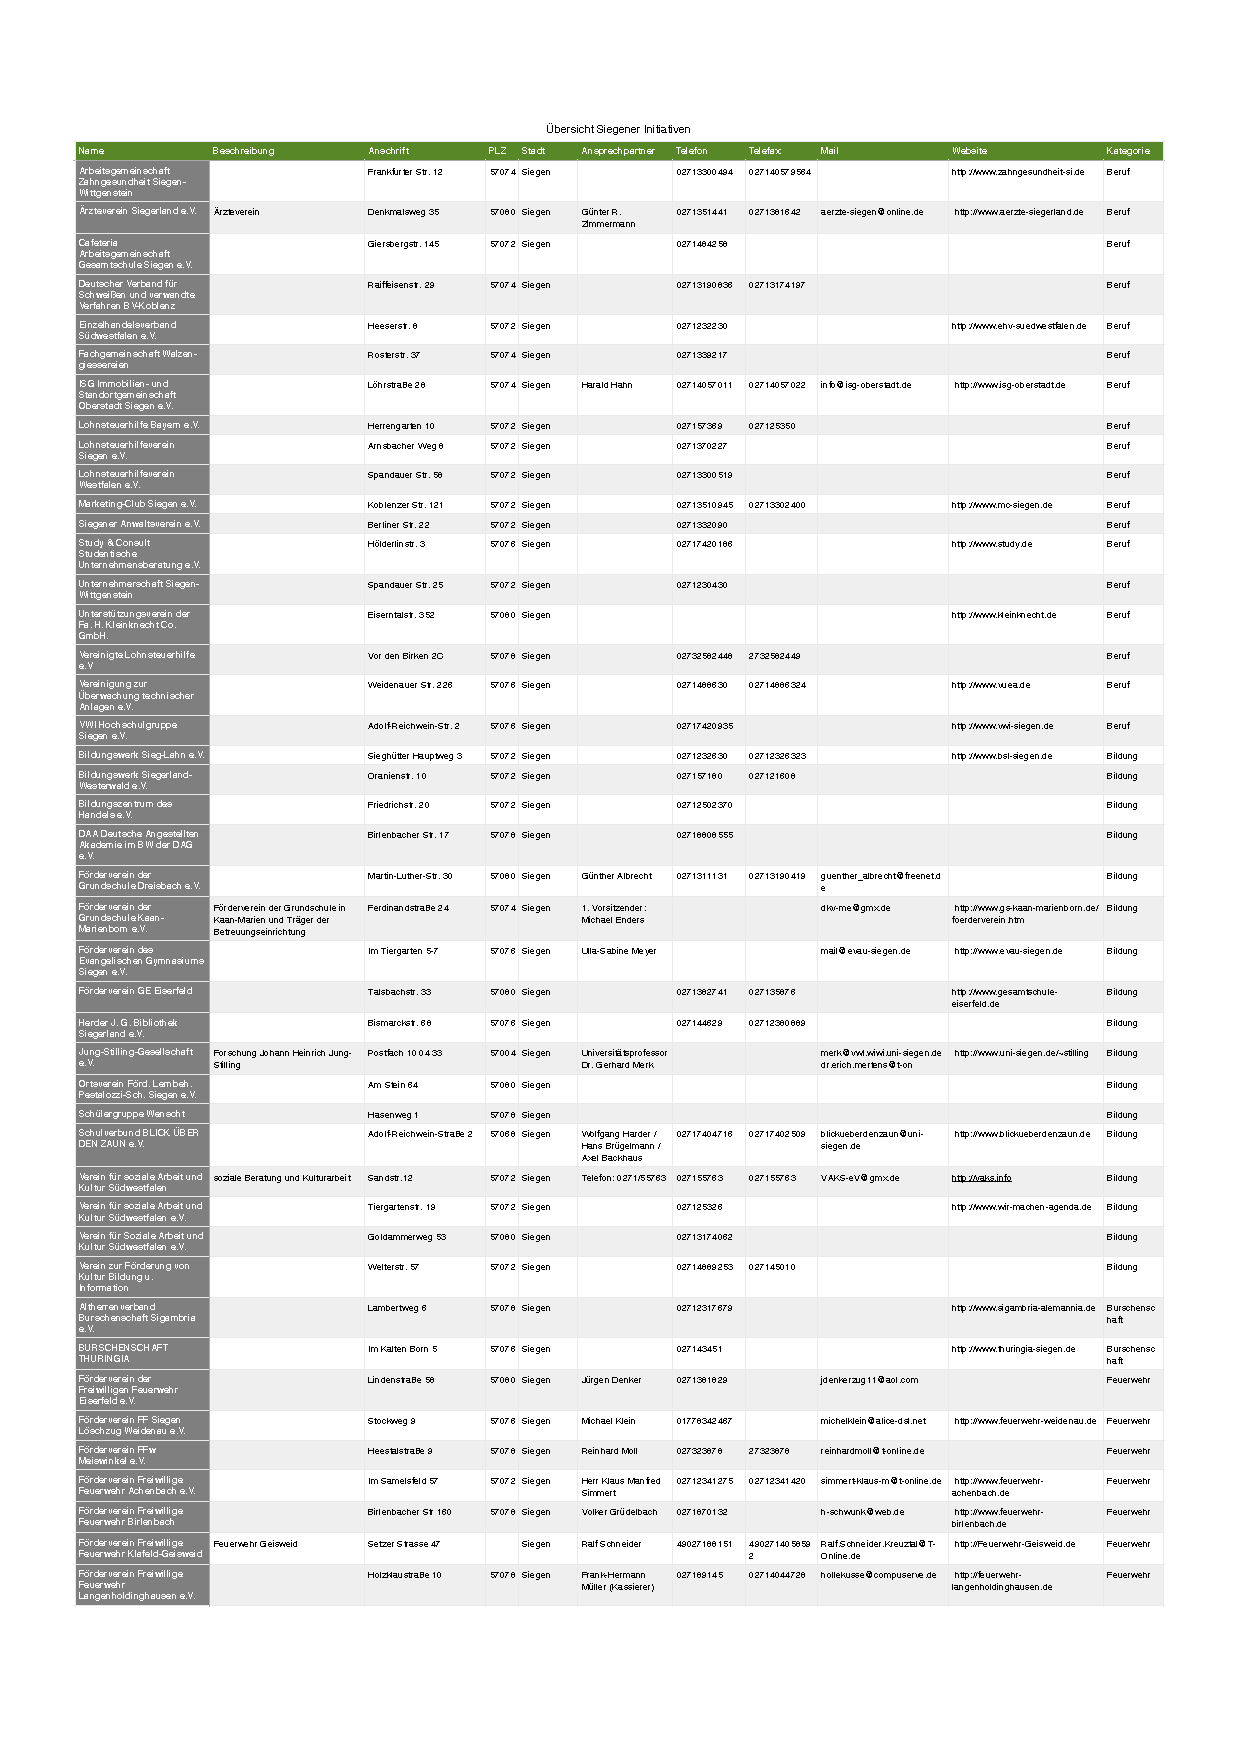
\includepdf[pages=-,pagecommand={\thispagestyle{plain}}]{/Users/Hybr1s/Documents/Uniarbeit/Vereinsforschung/Datenbank/SiegenerInitiativen.pdf}

%Die Methode der Kunst - Näherung von der Praxis
%Paul Feyerabend 
%\input{Kapitel/4.experiment.tex}
%Endergebnis: 
%Komme ich zu dem Schluss, dass eine Wissenschaft asugehend von der Kunst nicht möglich ist. Umgekehrt wäre es jedoch schon möglich: Wissenschaft als Kunst 

\end{document}